%% Document created 07 November 2021 automatically 
%% from /Users/massimosotgia/Desktop/uni_at_DIFI/Lab2/setup.py 

%% Copyright (C) Mattia Sotgia et al. 2022
%% Using class revtex4-2.cls
%                                       
%                                       
%██       █████  ██████         ██████  
%██      ██   ██ ██   ██             ██ 
%██      ███████ ██████          █████  
%██      ██   ██ ██   ██        ██      
%███████ ██   ██ ██████  ██     ███████ 
%                                       
%                                       
\documentclass[
    rmp,
    % preprint,
    % linenumbers,
    % tightlines,
    floatfix,
    reprint, 
    superscriptaddress, 
    altaffilletter, 
    amsmath, 
    amssymb, 
    a4paper]{revtex4-2}

\usepackage[top=1.75cm,bottom=2.5cm,left=1.5cm,right=1.5cm]{geometry}

\usepackage[utf8]{inputenc}
\usepackage[T1]{fontenc}

\usepackage[italian]{babel}

%% revtex4-2 bug-fix
\def\andname{e}
%--------------------
\makeatletter
\let\it@comma@def\active@comma
\makeatother

\usepackage{txfonts}
\usepackage{graphicx}% Include figure files
\graphicspath{{../fig/}}

\usepackage{dcolumn}% Align table columns on decimal point
\usepackage{bm}% bold math
\usepackage[colorlinks, urlcolor=., bookmarks]{hyperref}% add hypertext capabilities
\renewcommand\UrlFont{\color{blue}}

\usepackage{physics}
\usepackage{siunitx}

\usepackage{fancyhdr}
\pagestyle{fancy}
\fancyhf{}
\def\twodigits#1{\ifnum#1<10 0\fi\the#1}

%-----------------------------------------------------------------------------------------------

\usepackage{background}
\SetBgColor{gray}
\SetBgAngle{90}
\SetBgScale{2}
\SetBgVshift{0.27\textwidth}

\usepackage[american resistors]{circuitikz}
\usepackage{listings}
\lstset{
  basicstyle=\fontsize{5}{6}\selectfont\ttfamily,
  % backgroundcolor=\color{white},   % choose the background color
  % basicstyle=\footnotesize,        % the size of the fonts that are used for the code
  breakatwhitespace=false,         % sets if automatic breaks should only happen at whitespace
  breaklines=true,                 % sets automatic line breaking
  captionpos=b,                    % sets the caption-position to bottom
  % commentstyle=\color{mygreen},    % comment style
  deletekeywords={...},            % if you want to delete keywords from the given language
  escapeinside={\%*}{*)},          % if you want to add LaTeX within your code
  % extendedchars=true,              % lets you use non-ASCII characters; for 8-bits encodings only, does not work with UTF-8
  % firstnumber=1000,                % start line enumeration with line 1000
  % frame=single,                    % adds a frame around the code
  % keepspaces=true,                 % keeps spaces in text, useful for keeping indentation of code (possibly needs columns=flexible). 
  % keywordstyle=\color{blue},       % keyword style
  % numbers=left,                    % where to put the line-numbers; possible values are (none, left, right)
  % numbersep=5pt,                   % how far the line-numbers are from the code
  numberstyle=\tiny\color{gray}, % the style that is used for the line-numbers
  % rulecolor=\color{black},         % if not set, the frame-color may be changed on line-breaks within not-black text (e.g. comments (green here))
  showspaces=false,                % show spaces everywhere adding particular underscores; it overrides 'showstringspaces'
  showstringspaces=false,          % underline spaces within strings only
  showtabs=false,                  % show tabs within strings adding particular underscores
  stepnumber=2,                    % the step between two line-numbers. If it's 1, each line will be numbered
  % stringstyle=\color{mymauve},     % string literal style
  tabsize=2,                       % sets default tabsize to 2 spaces
}
\usepackage{soul}


%% Define ref types
\newcommand{\reftab}[1]{Tabella {\ref{#1}}}%
\newcommand{\reffig}[1]{Figura {\ref{#1}}}%
\newcommand{\refeqn}[1]{({\ref{#1}})}%
\newcommand{\ChiSqr}{$\chi^2$\space}
\newcommand{\ChiNdf}{$\chi^2/\text{ndf}$}
\newcommand{\cernroot}{\texttt{root}}
\newcommand{\treSigma}{$3\sigma$}
\newcommand{\stdErr}[1]{$\varepsilon_{#1}$}
\newcommand{\mstdErr}[1]{\varepsilon_{#1}}
%% PAPER ONLY custom Macros

\newenvironment{methods}[1]{\section*{#1}
%\fontfamily{phv}
\fontsize{7.5}{9}\selectfont\label{sec:methods}\noindent}{\par\noindent}

%\usepackage{lcsec}


\fancyfoot[C]{
    \the\year\twodigits\month\twodigits\day/3-\thepage
}
\fancyhead[C]{\fontfamily{phv}\fontsize{12}{12}\selectfont RELAZIONE DI LABORATORIO \textbf{
    N. 1 % ! <== CAMBIARE (Nessuna rel. -> 00)
    } (\the\year)
}

\begin{document}

\title{Misura della permeabilità magnetica relativa con circuito RLC risonante
}
\thanks{Esperienza n. 3
}

\author{Francesco Polleri}
\email{s5025011@studenti.unige.it}
\author{Mattia Sotgia}
\email{s4942225@studenti.unige.it}

\collaboration{Gruppo A1}
\affiliation{Dipartimento di Fisica, Università degli Studi di Genova, Italia}

\date{presa dati
    9 novembre 2021, consegnata in data
    19 novembre 2021
}

\begin{abstract}
    
\end{abstract}
\maketitle
\thispagestyle{fancy}
% Rimuovere per consegna
\SetBgContents{
    laboratorio2: e3 (non per la consegna) \today % ! Note di versione
}

%%%% CORPO DEL TESTO
%%%% CORPO DEL TESTO

\section*{Introduzione}\label{sec:introduction}
Si vuole misurare il valore della permeabilità magnetica di alcuni materiali dati, di cui non conosciamo esatta composizione chimico-fisica ma che possiamo ipotizzare omogenei, lineari e isotropi (LHI) fino al primo grado di approssimazione, avendo a disposizione un rocchetto plastico su cui sono avvolte $N$ spire di rame, nel quale può essere inserito il volume di materiale creato in modo da riempire quasi completamente il rocchetto. Variando il materiale ci aspettiamo di poter misurare i differenti valori della permeabilità magnetica $\mu_R$. 

Poiché i tipi di misure più precisi che siamo capaci a effettuare sono misure di tempo (in termini di periodo e di frequenza) sfruttiamo il circuito risonante RLC per determinare il valore della frequenza di taglio ($\nu_0$), che risulta legata al valore dell'induttanza e della capacità del condensatore. Cambiando il nucleo all'interno del solenoide modifichiamo il valore di $L$ e di conseguenza troveremo un valore differente di $\nu_0$. Dalla misura della frequenza troviamo il valore di $L$, essendo noti i valori delle altre componenti circuitali, e confrontando i diversi valori possiamo trovare $\mu_R$ per ogni materiale.

\begin{methods}{Metodi}
    \textit{Caratterizzazione del circuito RLC---} Il circuito RLC è definito da tre parametri: la frequenza di taglio $\nu_0$, il fattore di qualità $Q$ e il parametro $A$. Analizzando il circuito troviamo infatti che il valore della funzione di trasferimento è dato da \[\big|H[\nu]\big|=\frac{1}{\sqrt{1+\left(\frac{\omega L}{R} - \frac{1}{\omega RC}\right)^2}},\] per cui osserviamo che il suo valore massimo (cioè 1), si ottenga per $\omega=\omega_0=\frac{1}{\sqrt{LC}}$ che è il valore di quella che abbiamo chiamato frequenza di taglio ($\omega_0$ oppure $\nu_0$). Per valori più bassi e più alti di pulsazione e quindi di frequenza, il valore della funzione di trasferimento diminuisce, per cui il circuito si comporta come un filtro passa banda intorno al valore della frequenza di taglio che a seconda dei valori di L e di C del circuito può essere modificata. Allo stesso modo l'equazione della funzione di trasferimento può essere riscritta come \[\big|H[\nu]\big|=\frac{1}{\sqrt{1+Q_{id}^2\left({\nu\over\nu_0}-{\nu_0\over\nu}\right)^2}}\] dove Q è $Q_{id}=\frac{1}{R}\sqrt{\frac{L}{C}}$ (e abbiamo sostituito $\omega$ con $\nu = \omega / 2\pi$ dove $\nu=1 / T$), per cui notiamo che il filtro diventa tanto più selettivo, tanto più diventa grande Q, che viene definito quindi fattore di qualità. Inoltre dobbiamo anche considerare che l'induttanza si comporta in realtà anche come una resistenza, per cui dobbiamo riconsiderare il valore della funzione di trasferimento inserendo questo ulteriore parametro A uguale $A=\left(1+{R_L\over R}\right)^2$ da cui \begin{subequations}\begin{equation}\big|H[\nu]\big|=\frac{1}{\sqrt{A+Q_{id}^2\left({\nu\over\nu_0}-{\nu_0\over\nu}\right)^2}}.\label{eq:H(A, Q, v0)}\end{equation}
    
    Perciò in base ai valori di resistenza, capacità e induttanza che inseriamo all'interno del circuito possiamo modificare i valori di tali parametri. 

    Analogamente a quanto avviene per il modulo della funzione di trasferimento (in eq. \ref{eq:H(A, Q, v0)}), possiamo individuare la fase come \begin{equation}\varphi[\nu]=-\arctan(\frac{Q}{\sqrt{A}}\left({\nu\over\nu_0}-{\nu_0\over\nu}\right))\label{eq:phi(Q, A, v0)}\end{equation}\end{subequations}
    
    \begin{figure}[b]
        \begin{circuitikz}
            \ctikzset{bipoles/oscope/width=1.0}
            \draw (4.5,2)
            node[oscopeshape, fill=gray!20!white](O1){};
            \draw (O1.in 2) to [short, *-] (5.5,1.2) node[ground]{} node[below left]{GND};
            \draw (0,0)
            node[left]{$v_{in}=1$ V} node[below left=4pt]{(BNC in)} 
            to [short, o-] (0.5,0)
            to [L=$10$ mH, i_=$i$] (2,0)
            to [R=$R_L$, resistors/scale=0.4] (2.75,0)
            to [C=$220$ nF] (4,0)
            to [R=$38$ $\Omega$] (4,-2) 
            to [short] (0,-2)
            node[ground]{} node[left=4pt]{GND}
            (3.5,0) to [short, -] node[right]{$v_{out}$} node[below right=4pt]{(BNC out)} (4.5,0)
            to [short, -] (4.5,1.2)
            to [short, -*] (O1.in 1);
            \draw [red, dashed] 
            (-2,2) 
            node[align=left, below right=2pt]{Generatore di\\tensione\\alternata\\(Oscilloscopio)} 
            rectangle (0.5, -3);
        \end{circuitikz}
        \caption{Circuito utilizzato per il filtro passa-banda progettato nell'esperienza, i valori di R, L e C sono i valori nominali riportati sul componente. La resistenza $R_L$ è la resistenza interna all'induttanza, che verifichiamo non essere nulla.}
        \label{fig:circuit}
    \end{figure}
    
    
    \noindent\textit{Caratterizzazione dell'induttanza---}\label{par:L} La bobina su cui andiamo a eseguire le misure di $L$ è composta da un rocchetto cilindrico di plastica dura cavo, attorno al quale viene avvolto un filo di rame smaltato, a comporre 900 spire. L'apparato così creato si comporta come un solenoide caratterizzato da \begin{equation}\label{eq:inductance}L=\frac{\Phi_B}{I}=\mu_0\frac{N^2}{\ell}S\end{equation} con $\Phi_B=B\cdot NS$ il flusso del campo magnetico di un solenoide in cui scorre corrente $I$, dove consideriamo $n=N/\ell$ ottenendo che il solenoide è caratterizzato da \begin{equation}L=\mu_0 n^2 \ell S.\end{equation}
    Consideriamo, in primo ordine di approssimazione che il rocchetto di plastica abbia permeabilità magnetica pari a 1, valore che non si discosta molto dalla realtà sperimentale. 

    
    Inserendo un materiale all'interno del rocchetto ci aspettiamo una variazione del valore di $L$, dal quale vogliamo ricavare il valore di $\mu_R$ corrispondente al materiale. I materiali risultano avere dimensioni ($a\times a\times h$) uguali a $11.90\times11.90\times68.00$ mm (dimensioni del materiale A) e $12.10\times12.10\times68.00$ mm (secondo materiale, B). (Le misure sono riportate in Tab. \ref{tab:L_caratt}) Una volta inseriti nella cavità del solenoide non riescono però a riempirne completamente la superficie. Coprono invece tutta la lunghezza del solenoide, eccedendo rispetto al rocchetto, lungo 60.00 mm, di pochi millimetri, per cui ci riserviamo di non considerare effetti di bordo che richiederebbero calcoli non eseguibili sulla base dei dati raccolti.
    
    \begin{table}[h]
    \begin{ruledtabular}
        \begin{tabular}{lrl}
            Caratteristica & & \\
            Altezza solenoide & (60.0 & $\pm 0.1$)mm \\
            Diametro solenoide & (24.0 & $\pm 0.1$)mm \\
            Lato nucleo Fe (materiale A) & (12.10 & $\pm 0.05$)mm \\
            Altezza nucleo Fe & (68.00 & $\pm 0.05$)mm \\
            Lato nucleo Al (materiale B) & (11.90 & $\pm 0.05$)mm \\
            Altezza nucleo Al & (68.00 & $\pm 0.05$)mm \\
        \end{tabular}
    \end{ruledtabular}
\end{table}
    
    Dall'equazione \refeqn{eq:inductance} abbiamo che $L\cdot I=\Phi_B$. Quando inseriamo il materiale il flusso $\Phi_B$ si può ottenere come somma del flusso interno al materiale ed esterno (nello spazio tra il materiale e la bobina). Otteniamo quindi che  \begin{subequations}\begin{equation}L_{eq}= \frac{\Phi_B^\text{int}+\Phi_B^\text{ext}}{I}= \mu_0 n^2\ell\left(a^2\mu_R+\left(S-a^2\right)\right)=\mu_0n^2\ell\left(S+a^2\left(\mu_R-1\right)\right)\end{equation} dove $a^2$ indica la superficie di base del materiale considerato, con il fattore
    \begin{equation}\frac{\Phi_B^\text{int}}{I}=\mu_0\mu_Rn^2\ell a^2\end{equation} che tiene conto della permeabilità magnetica relativa del materiale e il fattore \begin{equation}\frac{\Phi_B^\text{ext}}{I}=\mu_0n^2 \ell\left(S-a^2\right)\end{equation}\end{subequations} che invece è il flusso fuori dal materiale.
        
    Da queste considerazioni otteniamo che quindi possiamo ricavare il valore della permeabilità magnetica $\mu_R$ come \begin{equation}\label{eq:mu_R}\mu_R=\frac{L_{eq}-\mu_0 n^2 \ell S}{\mu_0 n^2\ell a^2} + 1\end{equation}
        
    \noindent\textit{Scelta dei componenti del circuito---}\label{par:caratterizzazioneRLC} Vogliamo costruire un circuito la cui frequenza di taglio sia circa 3kHz in modo che intorno a questo valore di frequenza il segnale all'interno del circuito non sia disturbato da possibili rumori presenti a frequenze nell'ordine dei 100Hz o da altre interferenze presenti invece quando arriviamo a oltre 20KHz. Un'altra condizione che imponiamo è che il fattore di qualità sia almeno maggiore di 4 in modo che la banda che filtriamo attraverso il circuito sia sufficientemente stretta. Nello stesso momento vogliamo che questo fattore non sia troppo elevato perch\'e ci\`o renderebbe invece la banda troppo stretta, rendendo potenzialmente più difficile eseguire un fit dei dati. Inoltre il fattore di qualità, per come è stato definito, è legato ai valori di R, L e C, ma questi, per le condizioni in cui operiamo in laboratorio, cioè alle determinate frequenze descritte sopra, non permettono valori di Q elevati. 
    
    Dunque per il nostro progetto necessitiamo di particolari valori di R, C ed L. Quest'ultimo è già determinato, in quanto è legato alle caratteristiche fisiche del rocchetto di filo che appunto utilizziamo come induttanza. Quindi partendo da tale valore, che possiamo determinare in modo diretto usando il tester a nostra disposizione, ricaviamo anche quelli di R e C imponendo le condizioni sulla frequenza di risonanza e sul fattore di qualità. Se quindi vogliamo che $\nu_{0}=\frac{1}{\sqrt{LC}}\frac{1}{2\pi}$ sia pari a 3kHz, con L misurato grazie al tester che vale 10.03mH, allora $C=\frac{1}{L4\pi^2\nu_{0}^2}$ deve assumere un valore prossimo a 220nF. Prima di procedere a misurare R, attraverso la condizione su Q, misuriamo anche il valore della resistenza dell'induttanza, usando anche in questo caso il tester e otteniamo che $R_{L}$ è pari 3.7Ohm. Imponiamo che il valore di Q sia 6 e in base alla relazione $Q=\frac{1}{R}\sqrt{\frac{L}{C}}$ troviamo che $R=\frac{1}{Q}\sqrt{\frac{L}{C}}$, valore a cui però devo sottrarre quello di $R_{L}$ in quanto la $R_{eq}$ che ottengo dall'equazione precedente deriva in realtà dalla serie di R e $R_{L}$. Troviamo quindi che $R=\frac{1}{Q}\sqrt{\frac{L}{C}}-R_{L}$, cioè circa 38Ohm. In base ai valori trovati di R e C, cerchiamo tra i dispositivi presenti in laboratorio quelli che hanno valore nominale che più si avvicina a questi. Prendiamo quindi una capacità da 220nF e una resistenza da 38Ohm e misuriamo questi valori con il tester, per ottenere il loro effettivo valore. Quindi $C=(220\pm 2)nF$, $R=(38.0\pm 0.3)Ohm$ e $L=(10.0\pm 0.5)mH$.

    \noindent\textit{Presa dati---}Utilizziamo l'oscilloscopio come generatore di segnale in alternata che forniamo come input al nostro circuito. \hl{La frequenza di tale segnale \`e modificabile e il segnale di output del filtro cambia in base a tale frequenza.}
    
    Per individuare la frequenza di taglio del circuito misuriamo, sempre utilizzando l'oscilloscopio, la tensione in ingresso $v_{in}$, la tensione in uscita $v_{out}$, il periodo del segnale $T$ (uguale per entrambi i segnali in quanto sono isofrequenziali) e il ritardo tra i due segnali $dt$, con i rispettivi fondo-scala necessari per ricavare l'errore. 

    La prima cosa che facciamo è far variare la frequenza di $v_{in}$ per individuare il punto in cui il ritardo tra i due segnali è nullo, trovando quindi quella che dovrebbe essere $\nu_{0}$. A questo punto consideriamo un range di frequenze compreso tra una decade prima e una decade dopo il valore della frequenza di taglio e per ogni decade prendiamo tre misure di $v_{in}$, $v_{out}$, $T$ e $dt$ (ad esempio a 1kHz, 2kHz, 5kHz). Insieme a questi valori ne raccogliamo di ulteriori intorno a $\nu_{0}$.

    Ripetiamo questo procedimento tre volte, prima senza inserire alcun materiale all'interno dell'induttanza e poi aggiungendo uno per volta i due materiali che abbiamo a disposizione.
    
    I valori che abbiamo acquisito sono riportati nelle tabelle \ref{tab:rawdata_free}, \ref{tab:rawdata_m1} e \ref{tab:rawdata_m2}.
        
\end{methods}


\section*{Analisi dati}
Utilizziamo i dati raccolti per creare i grafici dei diagrammi di Bode della funzione di trasferimento e della fase. Per fare ciò calcoliamo $\big|H[\nu]\big|$ come rapporto tra $v_{in}$ e $v_{out}$ e la fase $\varphi$ come $2\pi\frac{dt}{T}$. Di conseguenza l'errore su $\big|H[\nu]\big|$ è dato da \[\mstdErr{|H|}=\sqrt{\left(\frac{\mstdErr{v_{out}}}{v_{in}}\right)^2+\left(\frac{\mstdErr{v_{in}}v_{out}}{v_{in}^2}\right)^2}\] mentre l'errore su $\varphi$ è pari a \[\mstdErr{\varphi}=2\pi\sqrt{\left(\frac{\mstdErr{dt}}{T}\right)^2 + \left(\frac{dt\cdot\mstdErr{T}}{T^2}\right)^2}\] 

Gli errori statistici di $v_{in}$, $v_{out}$, $T$ e $dt$ sono pari agli errori assoluti divisi per $\sqrt{3}$. Per trovare il valore degli errori assoluti cerchiamo sul data-sheet dell'oscilloscopio come calcolarli. % Alla fine quindi otteniamo
%\begin{subequations}\label{eq:errors_ds}
%   \begin{align}
    %    \mstdErr{v_{in}}  &= \frac{8  \cdot 0.035  \cdot (\text{fondo-scala}_{v_{in}} )}{\sqrt{3}} \\
   %     \mstdErr{v_{out}} &= \frac{8  \cdot 0.035  \cdot (\text{fondo-scala}_{v_{out}})}{\sqrt{3}} \\
    %    \mstdErr{T}       &= \frac{10 \cdot 0.0016 \cdot (\text{fondo-scala}_{T}      )}{\sqrt{3}} \\
     %   \mstdErr{dt}      &= \frac{10 \cdot 0.0016 \cdot (\text{fondo-scala}_{dt}     )}{\sqrt{3}}
   % \end{align}
%\end{subequations}


Creiamo quindi delle tabelle in cui riportiamo i valori di $\big|H[\nu]\big|$, $\varphi$ e $\nu$ con i rispettivi errori. Da tali tabelle costruiamo i grafici dei diagrammi di Bode per la funzione di trasferimento e per la fase. 


Per realizzare il fit di $\big|H[\nu]\big|$ utilizziamo l'equazione \refeqn{eq:H(A, Q, v0)} impostando come parametri $A$, $Q^2$ e $\nu_{0}$, mentre per la fase $\varphi$ utilizziamo l'equazione \refeqn{eq:phi(Q, A, v0)} impostando come parametri $\frac{Q}{\sqrt{A}}$ e $\nu_0$. Quindi, in base a come abbiamo definito questi parametri, considerando noti i valori assunti da $C$ e da $R$, possiamo ricavare il valore di $L$. Questo procedimento lo ripetiamo sia per la funzione di trasferimento che per la fase. Di conseguenza, da ognuno dei tre casi che stiamo considerando, avremo due valori di L. Se questi si rivelano compatibili, nei due casi in cui abbiamo inserito i materiali, procediamo a calcolare la miglior stima e da quest'ultimo valore, in base all'equazione \refeqn{eq:mu_R} troviamo $\mu_R$ del relativo metallo.

Nel primo caso(induttanza senza materiali al suo interno) il fit di $\big|H[\nu]\big|$ e quello di $\varphi$ ci restituiscono rispettivamente questi valori dei parametri: \hl{inserire valori}
Inserendo invece il materiale A i valori dei parametri sono: \hl{inserire valori}
Infine per il materiale B troviamo i valori ricavati sono: \hl{inserire valori}
\begin{figure*}
    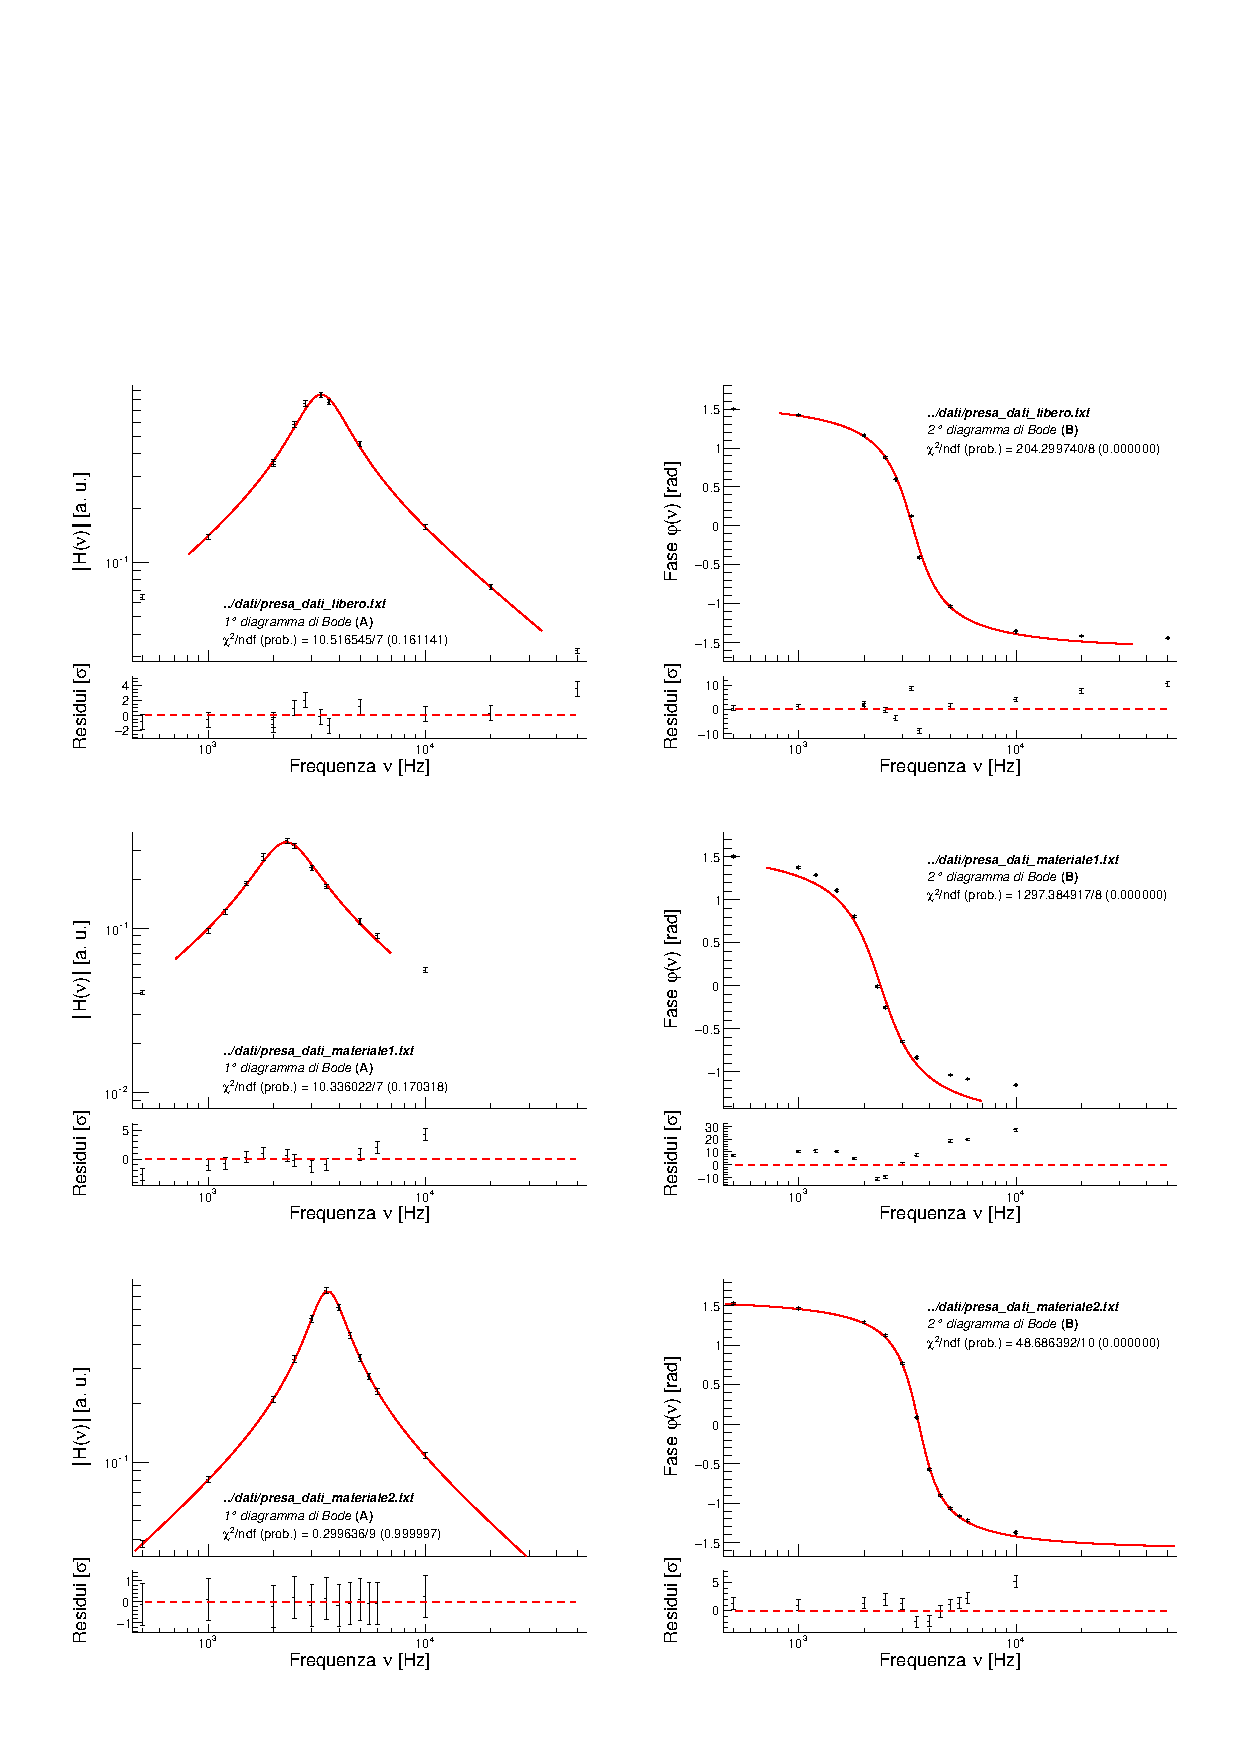
\includegraphics[width=\textwidth]{plot.pdf}
    \caption{Diagrammi di Bode per il filtro circuito RLC utilizzato. Gli assi sono allineati per evidenziare lo spostamento della frequenza di risonanza (picco della funzione di trasferimento) verso frequenze più basse per il materiale 1, e invece la quasi identità tra il caso libero e il secondo materiale, che possiamo quindi presupporre essere scarsamente magnetico, ovvero diamagnetico o paramagnetico (la distinzione richiede analisi più dettagliata del risultato in termini quantitativi). }
    \label{fig:plot}
\end{figure*}

\section*{Modello di fit su parametri circuitali}
Il modello prima usato sfruttava i parametri $A$, $Q^2$ e $\nu_0$ per la funzione di trasferimento e $\frac{Q}{\sqrt{A}}$ e $\nu_0$ per la fase, che sono però effettivamente derivati dai valori di $R$, $R_L$, $L$ e $C$, secondo le relazioni 
\begin{align}
    A &= \left(1\frac{R_L}{R}\right)^2 \\
    Q^2 &= \frac{1}{R^2}\frac{L}{C} \\
    \nu_0 &= \frac{1}{2\pi\sqrt{LC}} 
\end{align}
La funzione di trasferimento e la funzione della fase trovate in \refeqn{eq:H(A, Q, v0)} e \refeqn{eq:phi(Q, A, v0)} sono perciò effettivamente funzioni di $R$, $R_L$, $L$ e $C$ definite come
\begin{subequations}
    \begin{equation}
        \big|H[\nu]\big| = \frac{1}{\sqrt{\left(1+\frac{R_L}{R}\right)^2 + \frac{1}{R^2}\left(2\pi\nu L - \frac{1}{2\pi\nu C}\right)^2}}
    \end{equation}
    la fase e 
    \begin{equation}
        \varphi[\nu] = -\arctan(\frac{2\pi\nu L - \frac{1}{2\pi\nu C}}{R + R_L})
    \end{equation}
\end{subequations}


\section*{Considerazioni su errori a basse e alte frequenze}
Quando operiamo con valori di $\nu$ attorno a frequenze nell'ordine del 100Hz osserviamo visualmente sull'oscilloscopio che il segnale di $v_{out}$ è molto disturbato, per cui per misurare il suo valore ci affidiamo a una media operata dall'oscilloscopio. Nel fare questo passaggio dobbiamo quindi tenere conto che l'errore su queste misure è diverso da quanto ricaviamo per gli altri punti. Possiamo scegliere di procedere in due modi. Da una parte possiamo decidere di sovrastimare l'errore facendo misure \textit{a occhio} e quindi dare meno peso a questi punti nel fit. D'altra parte potremmo procedere invece con l'esclusione dal fit di tali punti. Scegliamo di procedere con quest'ultima opzione in quanto la prima non fornisce un risultato quantitativamente preciso e ci porta a fare un'alterazione dei dati raccolti, mentre la seconda lasca inalterati i valori numerici dei dati ed è in grado di fornirci un risultato più preciso. 

Un problema analogo si verifica quando i segnali oscillano ad alte frequenze (superiori a 50kHz, nell'ordine dei 100kHz). Il circuito viene realizzato su una base di lavoro (\textit{breadboard}) che presenta tante superfici conduttrici (necessarie per connettere i pin delle diverse componenti) che si possono comportare come capacità. Quando operiamo a basse frequenze il filtro, che si comporta come un passa alto, non risente dell'effetto di questi condensatori (che possiamo definire \textit{virtuali} all'opposto del condensatore \textit{reale}), mentre ad alte frequenze l'effetto può essere influente. 

Nel caso del solenoide libero il fit è ristretto da 800Hz fino a 35kHz, eliminando quindi due punti alle code. Nel caso del materiale A (nucleo di Fe) le problematiche descritte sopra sono evidenziabili sotto i 700Hz e sopra i 10kHz, per cui utilizziamo un range più ristretto per eseguire il fit. Nel caso del terzo materiale (nucleo di Al) non riscontriamo gli stessi effetti e quindi consideriamo tutti i punti raccolti. 

\section*{Considerazioni sull'errore legato al ritardo}
Osseviamo che i grafici relativi alla fase presentano un errore associato molto piccolo. Potremmo procedere considerando diversi metodi per compensare questa sottostima, eseguendo un processo di \textit{error scaling} oppure procedendo a ragionamenti legati agli errori nei valori alle code e nella condizione di risonanza. 

Per ottenere valori però sensati avremmo dovuto procedere già in sede di presa dati ad una considerazione di tipo statistico del ritardo e quindi ottenere relativamente a ogni frequenza un valor medio di $dt$ e deviazione standard. Questo processo sarebbe dovuto però essere in qualche modo previsto già in fase di progettazione e attuato nella presa dati considerando di automatizzare la presa dati e ottenere un set di dati più strutturato. 

Osservando quanto otteniamo dal valore del fit, non riteniamo opportuno però procedere neanche ad un ragionamento relativo allo \text{scaling} dell'errore, in quanto non osserviamo un moglioramento legato al cambio si fattore di scala. Gli errori quindi benchè sottostimati, sono tutti ricavati come in \refeqn{eq:errors_ds}.


\section*{Osservazioni sul comportamento del materiale A (nucleo di F\lowercase{e})}
Dai grafici in \reffig{fig:plot} possiamo osservare che la fase del nucleo di Fe ha un comportamento differente dagli altri due casi. Infatti senza aver bisogno di analizzare il fit possiamo notare che i valori ad alte frequenze tendono a una fase maggiore di $-\frac{\pi}{2}$, valore atteso dal modello utilizzato. Questo mostra come in realtà per questo caso il modello non sia corretto e giustifica il fatto che la funzione non riesca a eseguire il fit, e si ottenga un valore di \ChiNdf~ elevato. 

Un'altra conseguenza è legata al fatto che i parametri dai due fit non vengano compatibili, ed entrambi non portano a un risultato corretto. Scegliamo però comunque di portare a termine i calcoli per ottenere un valore di $\mu_R$, su cui possiamo fare ulteriori osservazioni. 

\begin{table}
    \begin{ruledtabular}
        \caption{Valori riferiti al grafico per il solenoide libero}
        \label{tab:plotdata_free}
        \begin{tabular}{ddd}
            
        \end{tabular}
    \end{ruledtabular}

    \begin{ruledtabular}
        \caption{Valori riferiti al grafico per il solenoide con il materiale A nel nucleo}
        \label{tab:plotdata_m1}
        \begin{tabular}{ddd}
            
        \end{tabular}
    \end{ruledtabular}

    \begin{ruledtabular}
        \caption{Valori riferiti al grafico per il solenoide con il materiale B nel nucleo}
        \label{tab:plotdata_m2}
        \begin{tabular}{ddd}
            
        \end{tabular}
    \end{ruledtabular}
\end{table}

\section*{Conclusioni}
% Dai valori ottenuti dai parametri, utilizzando le relazioni di definizione di $A$, $Q$ e $\nu_0$, torniamo ai valori di $R$, $L$ e $C$. Otteniamo però due valori per ogni caso, uno dalla fase e una dalla funzione di trasferimento. 

Dal fit eseguito otteniamo i valori dei parametri $A$, $Q$ e $\nu_0$ con i relativi errori. Otteniamo però due valori per ogni caso, uno dalla fase e una dalla funzione di trasferimento. 

Per il caso del solenoide libero troviamo la compatibilità tra i valori dei parametri entro \treSigma, quindi, considerando i set di dati essenzialmente scorrelati tra di loro (l'unica correlazione è legata al tempo, che però presenta errori molto piccoli, trascurabili quasi rispetto agli errori legati agli altri fattori) possiamo procedere a ricavare la miglior stima dei parametri, ottenendo quindi dalle relazioni di definizione di $A$, $Q$ e $\nu_0$ i valori di $R$, $L$ e $C$. 
Analizzando questi ultimi dati osserviamo, senza aver necessariamente bisogno di un calcolo rigoroso, che non risultano compatibili con quelli misurati in modo diretto usando il tester. Infatti i valori ottenuti sono \begin{align*}
    R &= 21.8\pm1.5 \Omega\\
    L &= 2.8 \pm 0.2 \text{mH}\\
    C &= 0.80 \pm 0.07 \mu\text{F}
\end{align*}
Osserviamo che comunque il fit ci restituisce ugualmente un rapporto costante di L e C che rispecchia il fatto che $\nu_0$ sia effettivamente simile al valore trovato direttamente quando abbiamo impostato che $dt$ fosse nullo.

In particolar modo definiamo $L_0$ il valore di $L$ ottenuto per questo caso: questo valore sarà necessario per calcolare il valore di $\mu_R$ relativo ai casi dove è presente il materiale nel nucleo, in quanto rappresenta il valore calcolato del modello privato di nucleo magnetizzabile.

Nel caso del materiale A, per i motivi descritti in precedenza, troviamo, come ci aspettavamo dei valori non compatibili tra i parametri trovati attraverso il fit della funzione di trasferimento e quello della fase. Quindi, non potendo fare la miglior stima, procediamo ricavando i valori di $R$, $L$ e $C$ in entrambi i casi e troviamo i valori riportati in \reftab{tab:rlc_m2}. Da questi valori troviamo due valori di $\mu_R$ che sono
\begin{align*}
    \mu_R^H &= 0.65 \pm 0.07 \\
    \mu_R^\varphi &= 3.0 \pm 0.6 \\
\end{align*}
Da questi valori ancora di più possiamo stabilire la non riuscita dell'esperienza, in aggiunta a osservare che il modello utilizzato non si adatta al comportamento del Fe. 

\begin{table}[h]
    \begin{ruledtabular}
        \caption{Valori di R, L e C ottenuti per il materiale A (Fe).}
        \label{tab:rlc_m2}
        \begin{tabular}{lrrr}
            Caso & Resistenza & Induttanza & Capacità \\
            & $R\pm\mstdErr{R}$ ($\Omega$) & $L\pm\mstdErr{L}$ (mH) & $R\pm\mstdErr{R}$ (nF) \\
            \colrule
            Risultati da $\big|H\big|$ & $1.87 \pm 0.14$ & $1.99 \pm 0.05$ & $(2.4 \pm 0.6)\times 10^3$ \\
            Risultati dalla fase  & $62 \pm 4$ & $8 \pm 5$ & $(6\pm4)\times10^2$ \\
        \end{tabular}
    \end{ruledtabular}
\end{table}

Nel caso del materiale B invece i valori dei paramatri risultano compatibili e dopo aver calcolato la miglior stima troviamo che i valori di $R$, $L$ e $C$ sono 
\begin{align*}
    R &= 11.2 \pm 0.8 \Omega\\
    L &= 2.50 \pm 0.01 \text{mH}\\
    C &= 0.79 \pm 0.07 \mu\text{F}
\end{align*}
In questo modo possiamo, dal valore di $L$, ricavare il valore di $\mu_R$. Dalla equazione \refeqn{eq:mu_R} otteniamo una relazione che lega $\mu_R$ con $L_{eq}$, ma possiamo osservare che $\mu_0n^2\ell S$ è proprio il valore del coefficiente di autoinduzione del circuito (in particolare del solenoide utilizzato) che però possiamo ottenere dal fit nel caso libero. 

% dalla equazione \refeqn{eq:mu_R}.  e otteniamo che però \hl{$\mu_R=0.86 +/- 0.08$} \st{valore che non ha alcun senso fisico, in quanto per come \`e definita $\mu_R$, pu\`o assumere solamente valori positivi.} Riguardando la formula utilizzata per trovare la permeabilità relativa e osservando il valore di $L$ in quest'ultimo caso dal fit, capiamo che il motivo per cui troviamo un valore negativo è dovuto al fatto che il programma ci restituisce un valore dell'induttanza troppo piccolo, in quanto è un ordine di grandezza più piccolo di quello che sarebbe dovuto essere secondo la misura diretta che abbiamo fatto. Notiamo infatti anche in questo caso che, come per il materiale A, il prodotto $L\cdot C$ rispecchia effettivamente il valore di $\nu_0$ ottenuto dal fit che è invece compatibile con quello che ci attendevamo in base ai valori di $L$ e $C$ inseriti nel circuito.

Per capire meglio quale possa essere il problema proviamo a ripetere l'analisi dati modificando però le funzioni di fit:\hl{inserire equazioni del secondo fit} in cui inseriamo direttamente come parametri i valori di $R$, $L$ e $C$ aggiungendo in più anche $R_L$. \hl{Notiamo che in questo caso}


% per materiale libero e Al si pu parlare della questione dell'errore di dt alla frequenza di risonanza, in qunato fissato lo zero il modello arctan() non può variare
% per il ferro discutere il problema della simmetria del modello, e della non simmetria dei dati rispetto allo zero. 



\begin{methods}{D\lowercase{ati completi e codice sorgente}}
    Tutti i dati completi a supporto dei grafici, e il relativo codice, sono visualizzabili su \url{https://github.com/mattiasotgia/Lab2}. L'analisi dati viene eseguita su un programma sviluppato in C++ basandosi su framework pubblici: ROOT, per la realizzazione dei grafici e il fit dei modelli (\url{https://root.cern/}).
\end{methods}


%\onecolumngrid
\appendix

% \setcounter{table}{0}
\renewcommand{\thetable}{S-\arabic{table}}
\begin{table*}[p]
    \begin{ruledtabular}
        \caption{Dati grezzi (induttanza libera)}
        \label{table:rawdata_free}
        \begin{tabular}{dddddddd}
            \multicolumn{2}{c}{Tensione ingresso (mV)} & \multicolumn{2}{c}{Tensione uscita (mV)} & \multicolumn{2}{c}{Periodo (ms)} & \multicolumn{2}{c}{Ritardo (ms)} \\
            v_{in} & range_{v_{in}} & v_{out} & range_{v_{out}} & T & range_T & dt & range_{dt} \\
            \colrule
            992.3  & 132 &  63.7 &  9 & 2      & 0.310  &  0.478  & 0.310  \\
            981.7  & 132 & 135.2 & 19 & 1      & 0.156  &  0.2267 & 0.156  \\
            907.4  & 132 & 320.2 & 45 & 0.5    & 0.078  &  0.093  & 0.078  \\
            907.4  & 132 & 327.2 & 44 & 0.5    & 0.078  &  0.0925 & 0.078  \\
            817.2  & 132 & 476.0 & 64 & 0.4    & 0.062  &  0.056  & 0.062  \\
            753.5  & 132 & 576.0 & 80 & 0.3571 & 0.056  &  0.034  & 0.056  \\
            559.5  &  80 & 475.7 & 68 & 0.303  & 0.050  &  0.006  & 0.050  \\
            601.6  &  86 & 467.0 & 66 & 0.2778 & 0.052  & -0.018  & 0.052  \\
            868.3  & 132 & 393.0 & 54 & 0.2    & 0.032  & -0.033  & 0.032  \\
            973.0  & 132 & 153.0 & 21 & 0.1    & 0.015  & -0.0216 & 0.015  \\
            981.7  & 132 &  72.0 & 10 & 0.05   & 0.0076 & -0.0113 & 0.0076 \\
            992.3  & 132 &  32.0 &  5 & 0.02   & 0.0030 & -0.0046 & 0.0030 \\
        \end{tabular}
    \end{ruledtabular}



    \begin{ruledtabular}
        \caption{Dati grezzi (materiale A)}
        \label{table:rawdata_m1}
        \begin{tabular}{dddddddd}
            \multicolumn{2}{c}{Tensione ingresso (mV)} & \multicolumn{2}{c}{Tensione uscita (mV)} & \multicolumn{2}{c}{Periodo (ms)} & \multicolumn{2}{c}{Ritardo (ms)} \\
            v_{in} & range_{v_{in}} & v_{out} & range_{v_{out}} & T & range_T & dt & range_{dt} \\
            \colrule
            990.6 & 140 &  40.3 &  6 & 2       & 0.320  &  0.480  & 0.320  \\
            973.7 & 140 &  94.4 & 14 & 1       & 0.168  &  0.219  & 0.168  \\
            960.0 & 156 & 121.1 & 20 & 0.8333  & 0.136  &  0.171  & 0.136  \\
            907.4 & 132 & 170.8 & 25 & 0.6666  & 0.108  &  0.1176 & 0.108  \\
            827   & 196 & 225.3 & 54 & 0.5556  & 0.098  &  0.0713 & 0.098  \\
            748.4 & 104 & 256.2 & 36 & 0.4327  & 0.070  & -0.0004 & 0.070  \\
            768.5 & 108 & 245.0 & 35 & 0.4     & 0.070  & -0.0163 & 0.070  \\
            838.0 & 132 & 195.7 & 31 & 0.3333  & 0.060  & -0.0346 & 0.060  \\
            882.3 & 124 & 159.0 & 23 & 0.2857  & 0.054  & -0.038  & 0.054  \\
            947.0 & 156 & 104.5 & 17 & 0.200   & 0.033  & -0.033  & 0.033  \\
            955.0 & 144 &  86.4 & 13 & 0.1667  & 0.030  & -0.0288 & 0.030  \\
            971.0 & 160 &  54.0 &  9 & 0.1     & 0.0164 & -0.0184 & 0.0164 \\
        \end{tabular}
    \end{ruledtabular}



    \begin{ruledtabular}
        \caption{Dati grezzi (materiale B)}
        \label{table:rawdata_m2}
        \begin{tabular}{dddddddd}
            \multicolumn{2}{c}{Tensione ingresso (mV)} & \multicolumn{2}{c}{Tensione uscita (mV)} & \multicolumn{2}{c}{Periodo (ms)} & \multicolumn{2}{c}{Ritardo (ms)} \\
            v_{in} & range_{v_{in}} & v_{out} & range_{v_{out}} & T & range_T & dt & range_{dt} \\
            \colrule
            996.0 & 164 &  37.9 &  6  & 2      & 0.340   &  0.4874 & 0.340  \\
            982.0 & 164 &  80.0 & 14  & 1      & 0.176   &  0.234  & 0.176  \\
            935.0 & 152 & 195.8 & 32  & 0.5    & 0.096   &  0.103  & 0.096  \\
            849.9 & 140 & 285.8 & 47  & 0.4    & 0.068   &  0.0715 & 0.068  \\
            704.2 & 116 & 381   & 64  & 0.3333 & 0.056   &  0.041  & 0.056  \\
            575.0 &  96 & 434.2 & 72  & 0.2857 & 0.052   &  0.004  & 0.052  \\
            646.9 & 108 & 400.6 & 66  & 0.250  & 0.045   & -0.0228 & 0.045  \\
            756.4 & 128 & 337   & 56  & 0.2222 & 0.039   & -0.032  & 0.039  \\
            838.6 & 140 & 286.5 & 47  & 0.2    & 0.033   & -0.034  & 0.033  \\
            887   & 148 & 242.5 & 40  & 0.1818 & 0.033   & -0.0337 & 0.033  \\
            910   & 152 & 209.3 & 36  & 0.1667 & 0.029   & -0.0324 & 0.029  \\
            972.0 & 156 & 105   & 17  & 0.1    & 0.0168  & -0.0218 & 0.0168 \\
        \end{tabular}
    \end{ruledtabular}
\end{table*}

\end{document}